\documentclass[sigconf]{acmart}

\usepackage{booktabs} % For formal tables
\usepackage{amsmath}
\usepackage{tipa}
\usepackage{subcaption}
\usepackage{graphicx}
\usepackage{hyperref}
\usepackage{parskip}
\usepackage{minted}
\usepackage{xcolor}
\usepackage{listings}
\usepackage{color}
 
\definecolor{codegreen}{rgb}{0,0.6,0}
\definecolor{codegray}{rgb}{0.5,0.5,0.5}
\definecolor{codepurple}{rgb}{0.58,0,0.82}
\definecolor{backcolour}{rgb}{0.95,0.95,0.92}
 
\lstdefinestyle{mystyle}{
    backgroundcolor=\color{backcolour},   
    commentstyle=\color{codegreen},
    keywordstyle=\color{magenta},
    numberstyle=\tiny\color{codegray},
    stringstyle=\color{codepurple},
    basicstyle=\footnotesize,
    breakatwhitespace=false,         
    breaklines=true,                 
    captionpos=b,                    
    keepspaces=true,                 
    numbers=left,                    
    numbersep=5pt,                  
    showspaces=false,                
    showstringspaces=false,
    showtabs=false,                  
    tabsize=2
}
 
\lstset{style=mystyle}

% Copyright
\setcopyright{none}
%\setcopyright{acmcopyright}
%\setcopyright{acmlicensed}
%\setcopyright{rightsretained}
%\setcopyright{usgov}
%\setcopyright{usgovmixed}
%\setcopyright{cagov}
%\setcopyright{cagovmixed}


% DOI
\acmDOI{ }

% ISBN
\acmISBN{ }

%Conference
\acmConference[DTU]{DTU conference}{August 2017}{Kgs Lyngby, Denmark} 
\acmYear{1997}
\copyrightyear{2017}


\acmArticle{1}
\acmPrice{3.50}

% These commands are optional
%\acmBooktitle{Transactions of the ACM Woodstock conference}
%\editor{Roar Nind Steffensen}


\begin{document}
\title{Report 3 - Operating Systems}
%\titlenote{Produces the permission block, and copyright information}
\subtitle{Roar Nind Steffensen (s144107)}
%\subtitlenote{The full version of the author's guide is available as
%  \texttt{acmart.pdf} document}


%\author{Ben Trovato}
%\authornote{Dr.~Trovato insisted his name be first.}
%\orcid{1234-5678-9012}
%\affiliation{%
%  \institution{Institute for Clarity in Documentation}
%  \streetaddress{P.O. Box 1212}
%  \city{Dublin} 
%  \state{Ohio} 
%  \postcode{43017-6221}
%}
%\email{trovato@corporation.com}

% The default list of authors is too long for headers.
%\renewcommand{\shortauthors}{B. Trovato et al.}


%\begin{abstract}
%This paper provides a sample of a \LaTeX\ document which conforms, somewhat loosely, to the formatting guidelines for ACM SIG Proceedings.\footnote{This is an abstract footnote}
%\end{abstract}

%
% The code below should be generated by the tool at
% http://dl.acm.org/ccs.cfm
% Please copy and paste the code instead of the example below. 
%
%\begin{CCSXML}
%<ccs2012>
% <concept>
%  <concept_id>10010520.10010553.10010562</concept_id>
%  <concept_desc>Computer systems organization~Embedded systems</concept_desc>
%  <concept_significance>500</concept_significance>
% </concept>
% <concept>
%  <concept_id>10010520.10010575.10010755</concept_id>
%  <concept_desc>Computer systems organization~Redundancy</concept_desc>
%  <concept_significance>300</concept_significance>
% </concept>
% <concept>
%  <concept_id>10010520.10010553.10010554</concept_id>
%  <concept_desc>Computer systems organization~Robotics</concept_desc>
%  <concept_significance>100</concept_significance>
% </concept>
% <concept>
%  <concept_id>10003033.10003083.10003095</concept_id>
%  <concept_desc>Networks~Network reliability</concept_desc>
%  <concept_significance>100</concept_significance>
% </concept>
%</ccs2012>  
%\end{CCSXML}

%\ccsdesc[500]{Computer systems organization~Embedded systems}
%\ccsdesc[300]{Computer systems organization~Redundancy}
%\ccsdesc{Computer systems organization~Robotics}
%\ccsdesc[100]{Networks~Network reliability}


%\keywords{Processes, Threads, System Calls, C}

\maketitle

The implementation for weeks 8, 9 and 10 will be uploaded in the zip file: \texttt{s144107skeletons89A.zip}.

\section{Week 8 - Synchronization}

%\begin{itemize}
    %\item Explain what mutual exclusion means.
    %\item How can semaphores be used to achieve mutual exclusion?
    %\item How can mutexes be used?
    %\item How can monitors be used?
    
    %In the example kernel and when running in kernel mode, interrupts are disabled. This makes it very easy to implement atomic actions.
    
    %\item How would you implement atomic actions if interrupts were enabled?
    %\item How would you implement atomic actions if you have multiple processors?
%\end{itemize}

\textbf{Mutual Exclusion}

When multiple actions access the same resources, and race conditions may occur, mutual exclusion is important to make sure, that the resources are handled properly. These kind of actions (or set of actions), are known as critical sections for the actor, which in our case could be an executing thread accessing a shared variable. If multiple actors have critical sections all needing to be mutually excluded, this is known as a critical region; a set of critical sections. 

Mutual exclusion, as implied in the text above, is the act of excluding all but a single member. Once the first has entered, any other member must wait for the first to finish before proceeding. This translates to our operating system by, at most letting a single thread be in a critical region at any time. In practice, several critical regions may exist, all protecting different shared resources, but for each critical region, mutual exclusion should be maintained to ensure the intended outcome. 

\textbf{Semaphores}

Semaphores are a great tool for restricting access and maintaining order. Semaphores work as a resource where the users never see what value the semaphore contains directly, only the consequences thereof. A semaphore is created with an initial value determined by the user. From here on, the user has two possible operations to perform on the semaphore; semaphore-down (\texttt{P}) or semaphore-up (\texttt{V}). These operations lower and raise the internal value some special amount respectively, with the amount depending on the implementation and use of the semaphore. A special thing about semaphores is, that the internal value is not allowed to be negative, meaning if a user tries to lower the value past zero, he will be denied. This is exactly the property which is harnessed for mutual exclusion, together with the fact that the two semaphore operations are themselves executed atomically (no interleavings with other operations). 

When a critical section is entered, a semaphore-down operation is performed. If the thread is not denied, the section is entered. When exiting the critical section, the semaphore-up operation is performed. That way other threads will be denied as long as the first thread is in the critical section, assuming that the semaphore was created with an internal value of 1, and the amount the internal value is incremented/decremented is by 1. 

Since semaphores may have any non-negative value in it's lifetime, it can be used for many other management implementations, such as a state where $n$ threads are allowed to be in at the same time, since the initial value of the semaphore determines how many semaphore-down operations are accepted before a semaphore-up operation is needed. 

\textbf{Mutexes}

The concept of mutexes is much like that of semaphores, if we only look at how semaphores are used for mutual exclusion. The mutex can be in one of two states; \textit{locked} and \textit{unlocked}. The operations on a mutex are called \textit{mutex\_lock} and \textit{mutex\_unlock}, and the effect of the operations are as the names imply. When a thread enters a critical section, they call \textit{mutex\_lock}. If the thread is denied it is blocked until the mutex is unlocked. Once the thread has entered the critical section and done the deed, \textit{mutex\_unlock} is called to free the mutex for other threads.

\textbf{Monitors}

The key concept of atomic actions are very important when dealing with shared resources. Semaphores and mutexes are good at handling this, but a more centralized strategy is to collect all access to the shared resources in one unit and make sure, that all procedures in that unit is handled as a critical region. This unit/object is called a monitor. 

Since the monitor has mutual exclusion, any thread trying to use the monitor while another thread is using it, is suspended until the monitor is free. This way the procedures inside the monitor does not suffer from race conditions. Monitors use constructs such as condition variables or condition queues to store the threads for synchronization, e.g. when trying to insert information into a buffer which is full. The condition variables have the the operations \textit{wait} and \textit{signal} which either stores or frees a thread in the respective variable. When a \textit{wait} operation is called, a suspended thread waiting to enter the monitor is granted access. 

When a thread calls the \textit{signal} operation two things may occur depending on the implementation of the monitor. Either the calling thread continues in the monitor, or the signalled thread continues in the monitor. Since a monitor is dependent on mutual exclusion, both threads are not allowed to both proceed in the monitor. Both solutions are possible, but according to the book Modern Operating Systems \cite{tanembaum} section 2.3.7, Brinch Hansen found that the prior solution was desired as long as the signal came as the last statement in the monitor, merging the signal and exiting the monitor.

\textbf{Atomic actions with interrupts enabled}

The operating systems implemented in the labs so far is a non-preemptive system with interrupts disabled. This means that all implementation of the kernel is handled as atomic actions, as the control flow will only change if explicitly told so. With interrupts enabled, we need to implement mutual exclusion in order to ensure that the actions are not interrupted. This could be done by implementing the specific actions as procedures in a monitor if possible, but since C does not support monitors, mutexes could be used instead. The action would be handled as a critical section and surrounded with the \textit{mutex\_lock} and \textit{mutex\_unlock} operations.

\textbf{Atomic actions with multiple processors}

Defining critical regions across multiple processors, means that there must some sort of communication between the processors. Either a specific memory location is specified for a lock in memory (if the processors have access to the same memory) or directly on disk. Since this lock presumable will be used often, disk would not be recommended as it would be highly inefficient. Hardware support, in the form of dedicated cache memory shared between the processors for the lock, would be a good way to solve the problem. For atomic lock operations, \texttt{TSL} (Test-and-Set-Lock) operations is often the preferred choice. This also needs hardware support to make the \texttt{TSL} operations atomic. \texttt{TSL} works by settings the value of the lock to \textit{locked} and returning the initial value of the lock. When the critical region is exited, the lock is set to \textit{unlocked}, much like the previous discussed cases.

\textbf{Lab implementation of semaphores}

Semaphores are implemented with a data structure much like the processes and threads. A global array of structs is initialized with 256 elements, using the macro \texttt{MAX\_SEMAPHORES} in the file \texttt{kernel\_customization.h}. A semaphore is defined by its internal value operated on by the semaphore-up and semaphore-down operations. The semaphore also has a flag stating if it is currently in use (called \texttt{used}) and a pointer to the owning process. The \texttt{used} flag is used when creating semaphores, distinguishing between free and occupied semaphores. Since semaphores should only be accessible from inside the owning process, the process pointer is checked when ever a semaphore is referenced, together with the \texttt{used} flag. When a semaphore-down operation is called on a semaphore with an internal value of zero, the system call could either block the thread or return an error. Returning an error means that a thread trying to gain access to a critical region would need to perform a busy wait, which is unwanted. 

When a semaphore is created, calling the \texttt{createsemaphore} system call a semaphore not in use is found and initialized; setting the internal value to the specified parameter given on the \texttt{edi} register, marking it as used and setting the process pointer to the current threads process' address. For the semaphore-up and down operation, if the semaphore's process pointer and \texttt{used} flag is not as expected, \texttt{ERROR} is returned. For the semaphore-up operation the internal value is then incremented followed by a search through the threads. If a thread is found, who's process is the semaphores process and is waiting for that exact semaphore, the thread is unblocked. For the semaphore-down operation, the internal value is checked for zero. If it is zero, the thread is blocked and the thread is set to yield, allowing other threads to leave the respective critical region. If the value is non-zero, it must be positive, and the internal value is decremented and the thread may proceed.

This implementation utilizes that interrupts are disabled during system call executions in the kernel, and therefore mutually excluded. 
\section{Week 9 - Memory}

%\begin{itemize}
    %\item In the system, memory can only be allocated in sizes of an even multiple of four kilobytes. What are the possible reasons for that?
    %\item In your implementation, memory is maintained using a bitfield structure. What would the differences be if a linked list structure is used?
    %\item What are the advantages and disadvantages of using a linked list structure?
%\end{itemize}

\textbf{Memory allocation in multiples of four kilobytes}

Discretizing memory into contiguous blocks, is a way to create an abstraction from direct addresses to a block of memory. This makes memory management more efficient, since only free/allocated blocks must be evaluates instead of every address themselves. Large blocks means fewer blocks to evaluate and faster memory management, but too large blocks results in inefficient use of memory. There is therefore a compromise between speed and how well memory can be utilized.

Blocks of memory is used in memory management algorithms such as page tables and virtual memory, where the the table sizes depend on the block sizes. As memory can be needed in various quantities, no optimal choice of memory block sizes exists, as it depends on the programs running. Empirically 4 kB works efficiently and works as a good compromise between speed and memory usage.

When evaluating block sizes with respect to cache, it is useful to have block sizes which divides the cache size without remainder. Otherwise the remaining cache would never be used. The cache sizes are in general a power of two, meaning it is divisible by 4 kB $= 2^{12}$ bytes, as long as cache is larger than 4 kB.

\textbf{Bitfield vs Linked list structure}

For memory management, there are in general two ways to keep track of memory; bitfields (also known as bitmaps) and free lists, as stated in the book Modern Operating Systems section 3.2.3 \cite{tanembaum} and seen in figure \ref{fig:mapvslist}. Both strategies divide memory up into page frames/indivisible chunks and manage the frames themselves. For a bitfield, a table is stored with information regarding to whether each frame is free or used. Additional information (as seen in the labs), may be stored in the table, such as what processes owns the used frames and the first frame of the block of allocated set of contiguous frames. Allocating memory using a bitfield is achieved by finding the needed free contiguous entries in the table. With a bitfield once memory is freed next to already free memory, the border between them disappears automatically, creating one large section of free memory. This means that no further operations are performed to merge free sections of memory, as compared to the linked lists structure.

\begin{figure*}
    \centering
    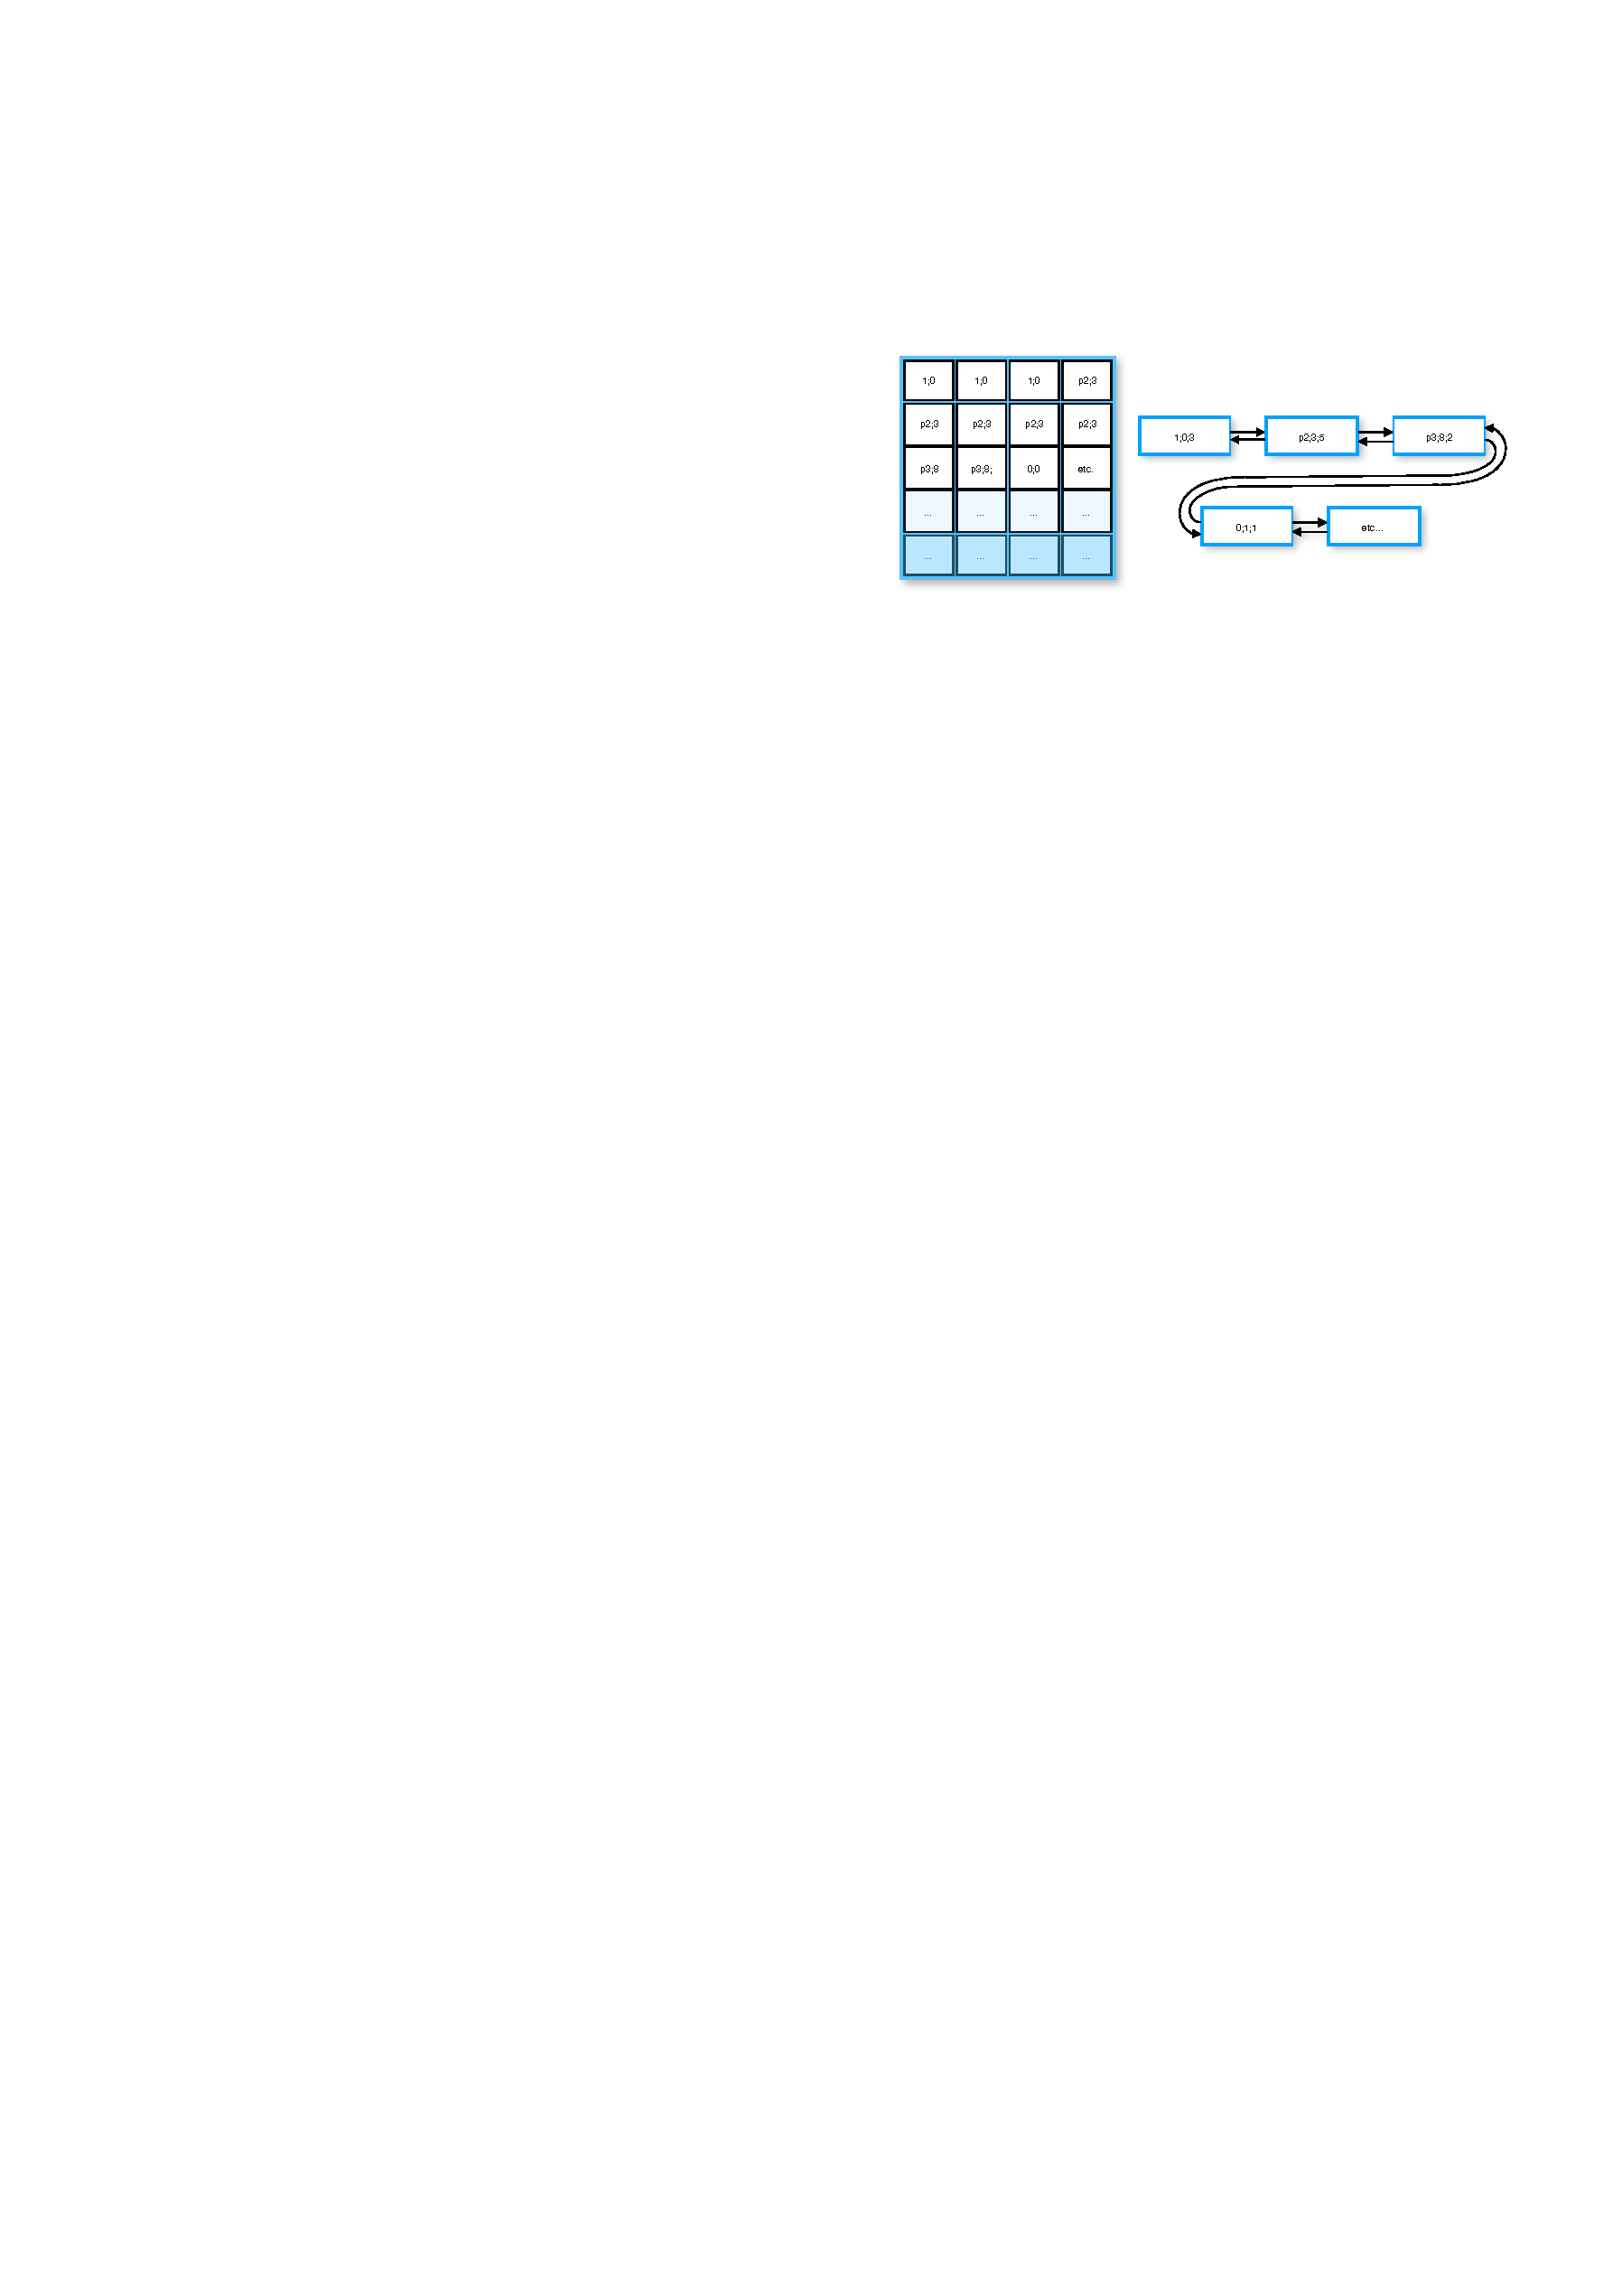
\includegraphics[width=0.7\textwidth]{fig/bitmatvslist.pdf}
    \caption{A bitmap/bitfield and a linked list representation of the same memory. The bitmap elements consist of a process pointer (where 1 is kernel and 0 is free) and a start index. The linked list elements consist of a process pointer, a start index and block size (together with pointers).}
    \label{fig:mapvslist}
\end{figure*}

When memory is managed with a linked list, each entry of the list contains four values; the process using the memory (if allocated) or a hole (if free), the starting index of the section, the size of the section and a pointer to the next element in the list. This way, when memory is allocated, the list is traversed and once an element corresponding to a hole of the correct size (most similar, first or largest depending on the allocation strategy, discussed further in the book \cite{tanembaum} section 3.2.3) is found, the memory is allocated. Finding memory slots may therefore be easy with a list, but once memory is freed, there is a risk of getting fragmented memory. When memory is freed, and the memory next to it is free also, they must be merged to one element in the list. For better performance, a double linked list may be preferred, to check the element before it in the list. Likewise when memory is allocated and a hole of larger size is found, it must be split into the allocated memory and a hole of remaining size.

Since the linked list dynamically creates elements at runtime, it must be possible to allocate memory for the elements themselves, meaning that special memory management for the list data structure must be available. Since the bitfield is of constant size, this problem does not occur, although the bitfield in general will use more memory, multiple entries in the table may hold the same information, as compared to the list.

\textbf{Lab implementation of page frames}

The kernel is set up with an array of page frames corresponding to the available memory for the system. The kernel itself uses a portion of these page frames, and these page frames are set as used and not deallocatable, meaning that no other process can accidentally or maliciously deallocate and overwrite kernel memory. The page management is implemented in the system calls \texttt{allocate} and \texttt{free}, which respectively allocates a set of contiguous free pages of a specified size, or frees an allocated memory block given the start page address from the block.

When allocating memory it is therefore necessary to first calculate the needed amount of pages to account for the requested amount of bytes, and find a spot of contiguous page frames in the page frame table. If such a spot in the page frame table is found, the members of the pages themselves are updated with respect to the start of the block and calling process, and an address to the allocated memory is returned. If no spot in the table is large enough \texttt{ERROR} is returned.

When freeing a memory block, we first want to be make sure that the complete block is allowed to be deallocated. The table is checked starting at the head of the block and continuing as long as the the page frames refer to the head of the block as the start of their block. If all page frames in the block are allowed to be freed, their owner and start index is reset, otherwise, if just a single page frame in the block is owned by another process or is not deallocatable, \texttt{ERROR} is returned and the memory is unchanged.
\section{Week 10 - Message passing}


%The message passing scheme implemented in this task is rendezvous.

%\begin{itemize}
    %\item  What might be the motivation behind this design?
    %\item Are there any drawbacks?
    
%Processes in an operating system should be isolated from each other to prevent one badly written or malicious process from destabilizing the whole system. Any process can communicate on a port as long as it knows its index.
    
    %\item Briefly outline a scheme in which each process is given private port identifiers, i.e., identifiers or handles which can only be used by the process that obtained them.
%\end{itemize}

\textbf{Rendezvous}

Using a rendezvous scheme for message passing, means that synchronous message passing can be implemented in a simple manner. 

For rendezvous, no buffer is needed, as the message/data is injected directly from one process' address space into the other. This means, that both processes are synchronized during the data transfer. The process sending the message will therefore be blocked until the receiving process is ready, vice versa if the receiving process calls before the sending process.

Since the processes are synchronized when a message is transferred, deadlocks may occur. Two processes trying to receive a message will halt the system. This is not optimal, but a direct consequence from the rendezvous scheme. Likewise a deadlock could occur if both processes were waiting to receive a message.


\textbf{Message passing with private process identifiers}

This question can be interpreted in two ways:
\begin{enumerate}
    \item Processes can be given identifiers to other processes' ports but the identifiers are not globally available.
    \item No process can obtain the identifier of another process' port identifiers.
\end{enumerate}

\underline{For the first scenario:}

If the message passing between processes is limited to the identifiers obtained for each process, the possible channels can be written as a graph, where there are not edges between all vertices. This would lead way for specific protocols, as the messages had to follow the structure defined in the graph (dictated by the obtained interprocess port identifiers). If the \texttt{receive} command is implemented as in the labs, the edges in the graph would be bidirectional, as the receiver would obtain the identifier for the sending process in the \texttt{sender} parameter and if the port identity is known/follows a known pattern, e.g. 0 and incrementing.

\begin{figure}
    \centering
    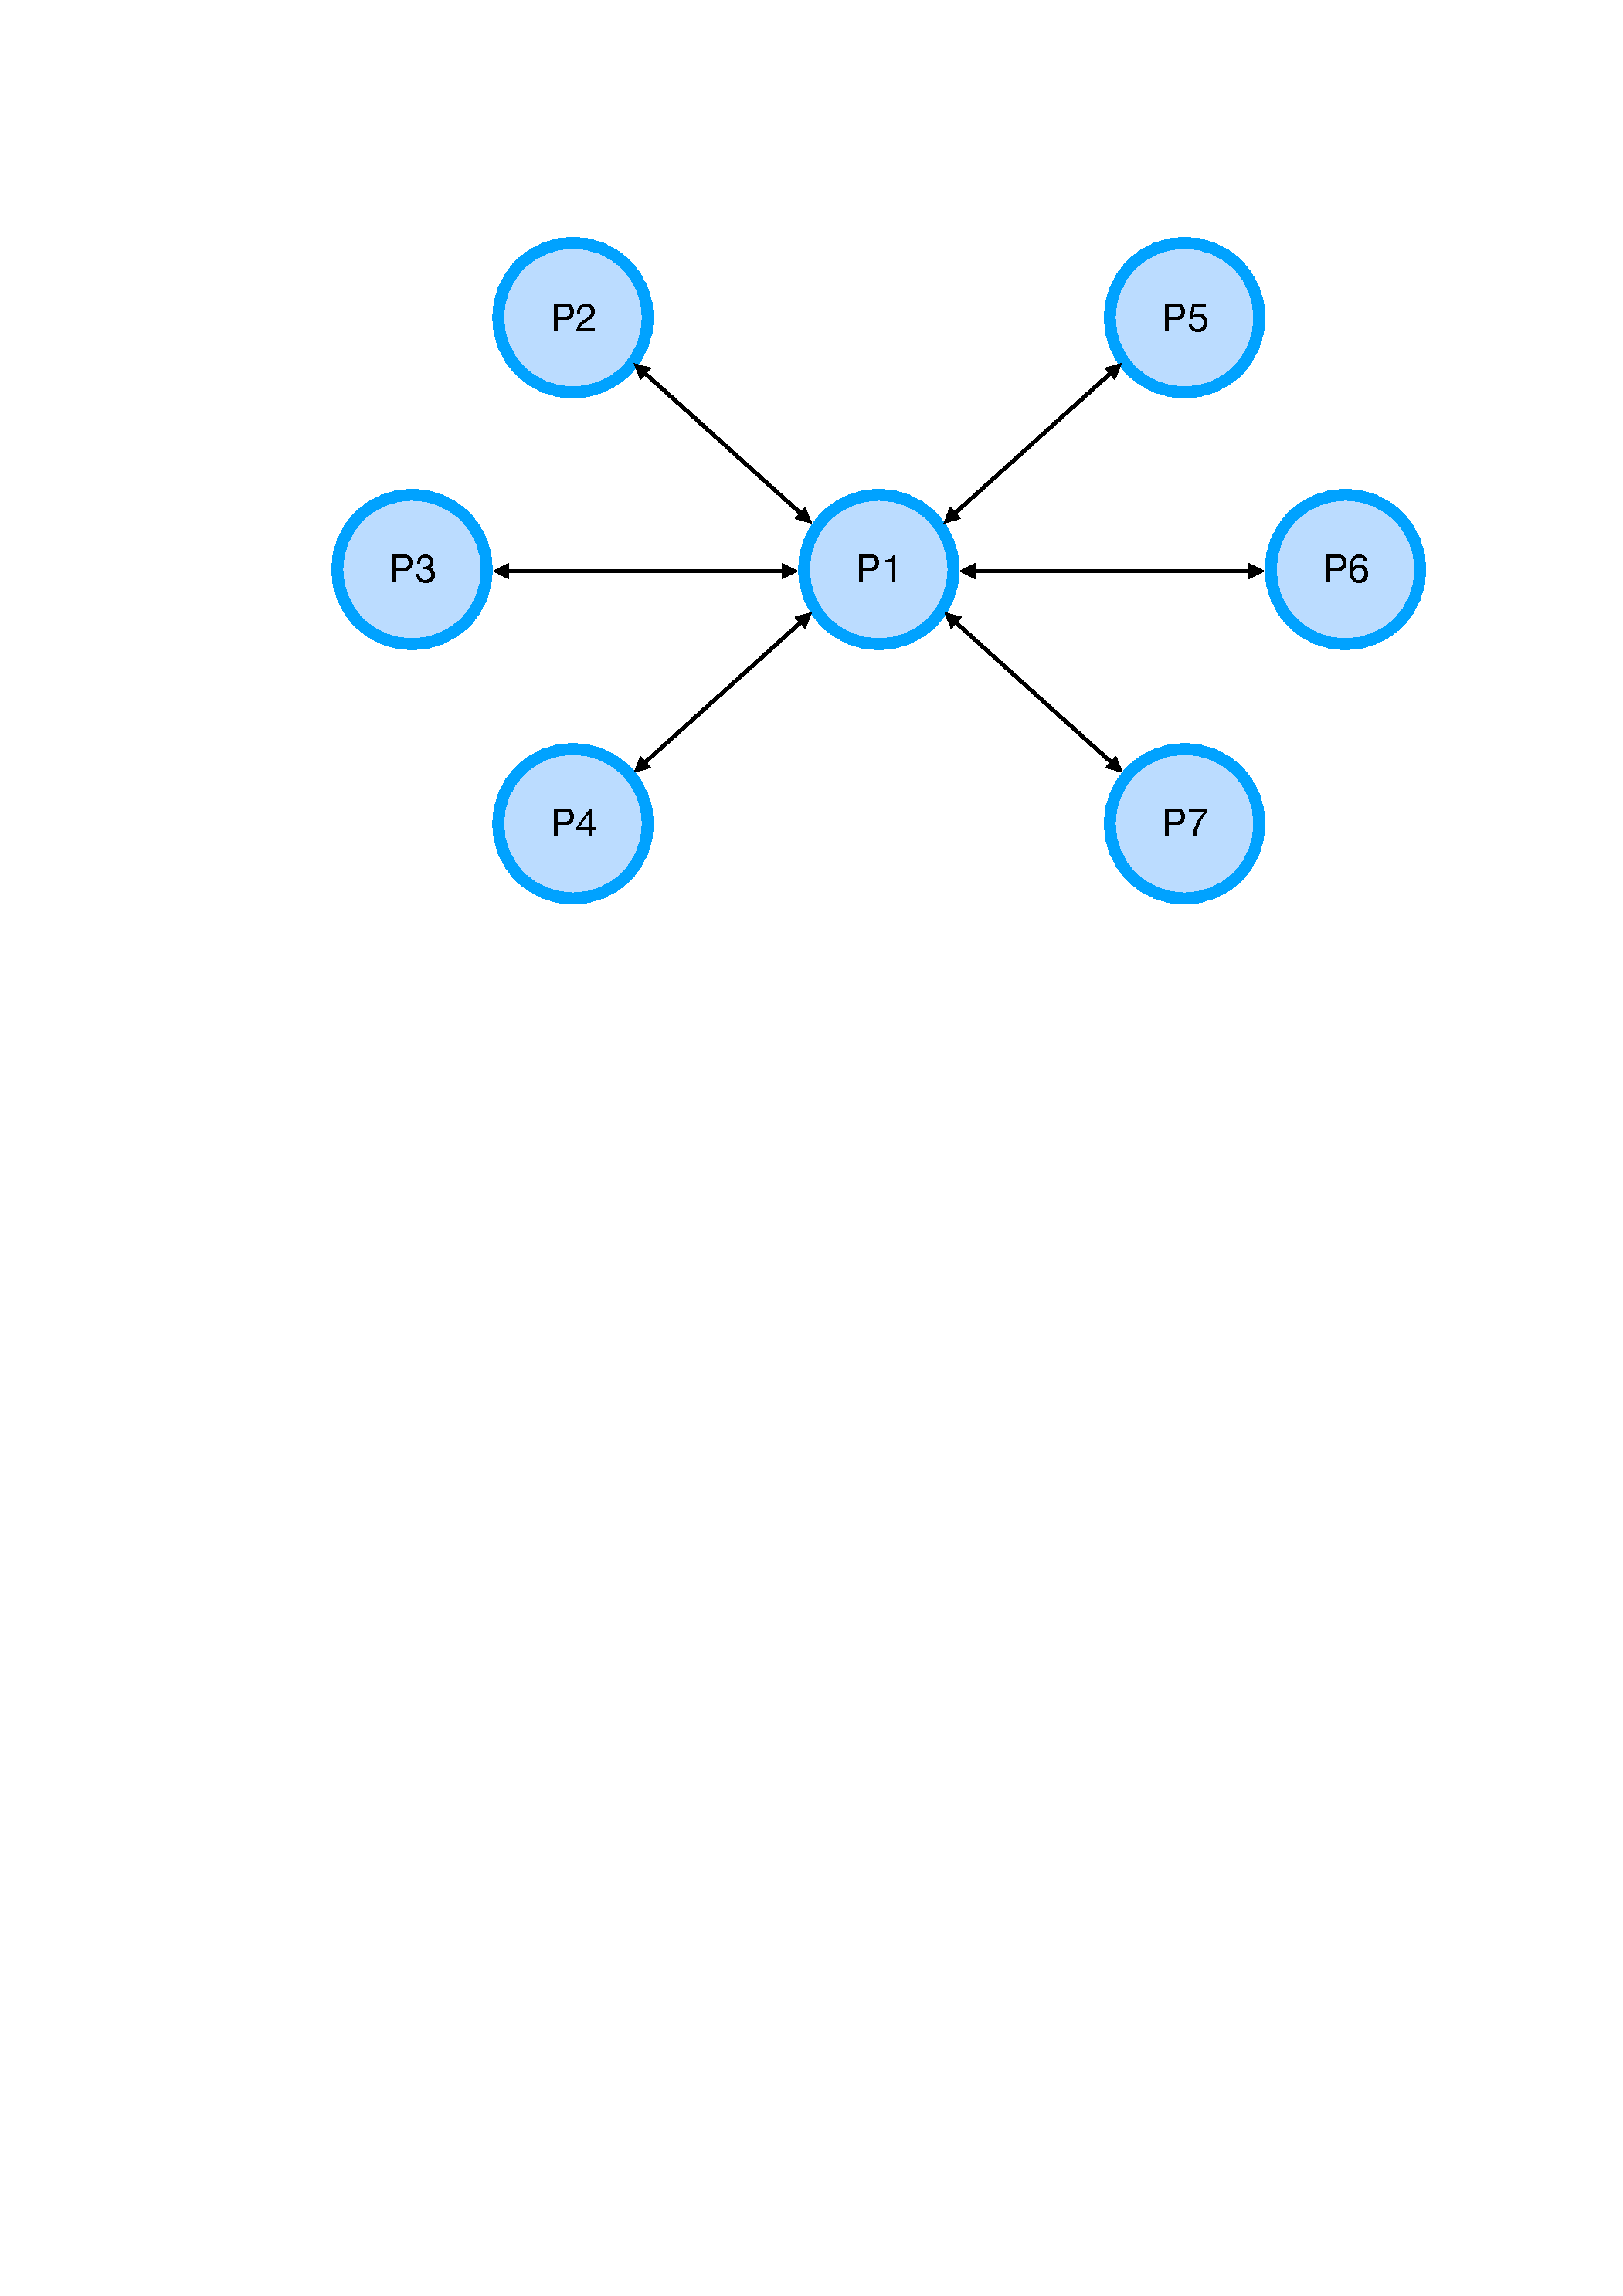
\includegraphics[width=0.7\linewidth]{fig/processGraph.pdf}
    \caption{A graph describing possible channels for message passing between processes with private port identifiers, following scenario 1. The example shows a conductor able to synchronize several processes which are not allowed/able to share information between themselves.}
    \label{fig:conductorGraph}
\end{figure}

This would be efficient if several users were using the same system, and were not allowed any form of interaction, of if several processes needed a conductor but are not allowed to share information between them. Such as graph can be seen in figure \ref{fig:conductorGraph}.

\underline{For the second scenario:}

Restricting process port information to the process itself would result in only threads from that process being able to send and receive messages between them. No two processes would be able to send/receive messages between them, and the message passing concept is therefore unnecessary, as the information and synchronization could be implemented using semaphores with shared variables, or a monitor if available in the language. With that said, the interthread message passing might lead to simpler solutions and higher performance, although it would mean a process should send messages to it's own port, meaning this should be supported by the system.

\textbf{Lab implementation of rendezvous message passing}

The message passing is implemented through the system calls; \texttt{findport}, \texttt{send} and \texttt{receive}. 

The system call for finding a port takes a port identifier and a process identity as parameters. These values correspond to the \texttt{id} of the port inside the process, and the index of the process in the process array. The ports are searched through to find a match. If a match is found, the identity for the port is returned. If no match is found, \texttt{ERROR} is returned.

When sending/receiving, one of two scenarios happens: either there is a corresponding process anticipating a receive/send in which case the rendezvous can occur, otherwise that thread of the process is blocked until further notice. Blocking threads in this case, is managed through two port pointers called \texttt{sending} and \texttt{receiving}. These pointers inform the scheduler if they are currently anticipating a send/receive (by not being null) and contain information as to what port it is waiting for, when the opposing process participates in the rendezvous. The system calls for sending and receiving are very similar; first the corresponding port pointer is set by the specified port handler given as a parameter in the \texttt{edi} register, the \texttt{sending} pointer for \texttt{send} and \texttt{receiving} for \texttt{receive}. The threads are then searched through for a match, equivalent to a thread who is anticipating the rendezvous on the same port, if a match is found the message is transferred between the two processes' address spaces.

The information contained in the message sent, is copied into the declared variable pointed to by the parameter specified on the \texttt{esi} register, meaning that the processes' address spaces never overlap, information is only send from one address space to another during the system call.

When the rendezvous has occurred their port pointers sending and receiving is set to null telling the scheduler that they are no longer blocked.

If no match was found, which would be the case for the initial \texttt{send}/\texttt{receive} call, the thread's port pointer is still set to the specified value and is set to yield, resulting in a block until the rendezvous can proceed.


\bibliographystyle{ACM-Reference-Format}
\bibliography{sample-bibliography} 

\end{document}
